\documentclass{article}
\usepackage[utf8]{inputenc}

% Page setup
\usepackage[a4paper,landscape,margin=2cm]{geometry}
\usepackage{amsmath}

% Typography
\usepackage[scaled]{helvet}
\let\familydefault\sfdefault

\usepackage[usenames,svgnames]{xcolor}
\usepackage{tikz,pgfplots}
\usetikzlibrary{positioning,arrows,intersections}

\definecolor{colordelta}    {RGB}{199,212,104}
\definecolor{colorsnapshot} {RGB}{79 ,142,209}
\definecolor{colordict}     {RGB}{143,232,186}
\definecolor{colorhdt}      {RGB}{49 ,167,226}
\definecolor{colortext}     {RGB}{29 ,29 ,27 }

\begin{document}
\pagestyle{empty}
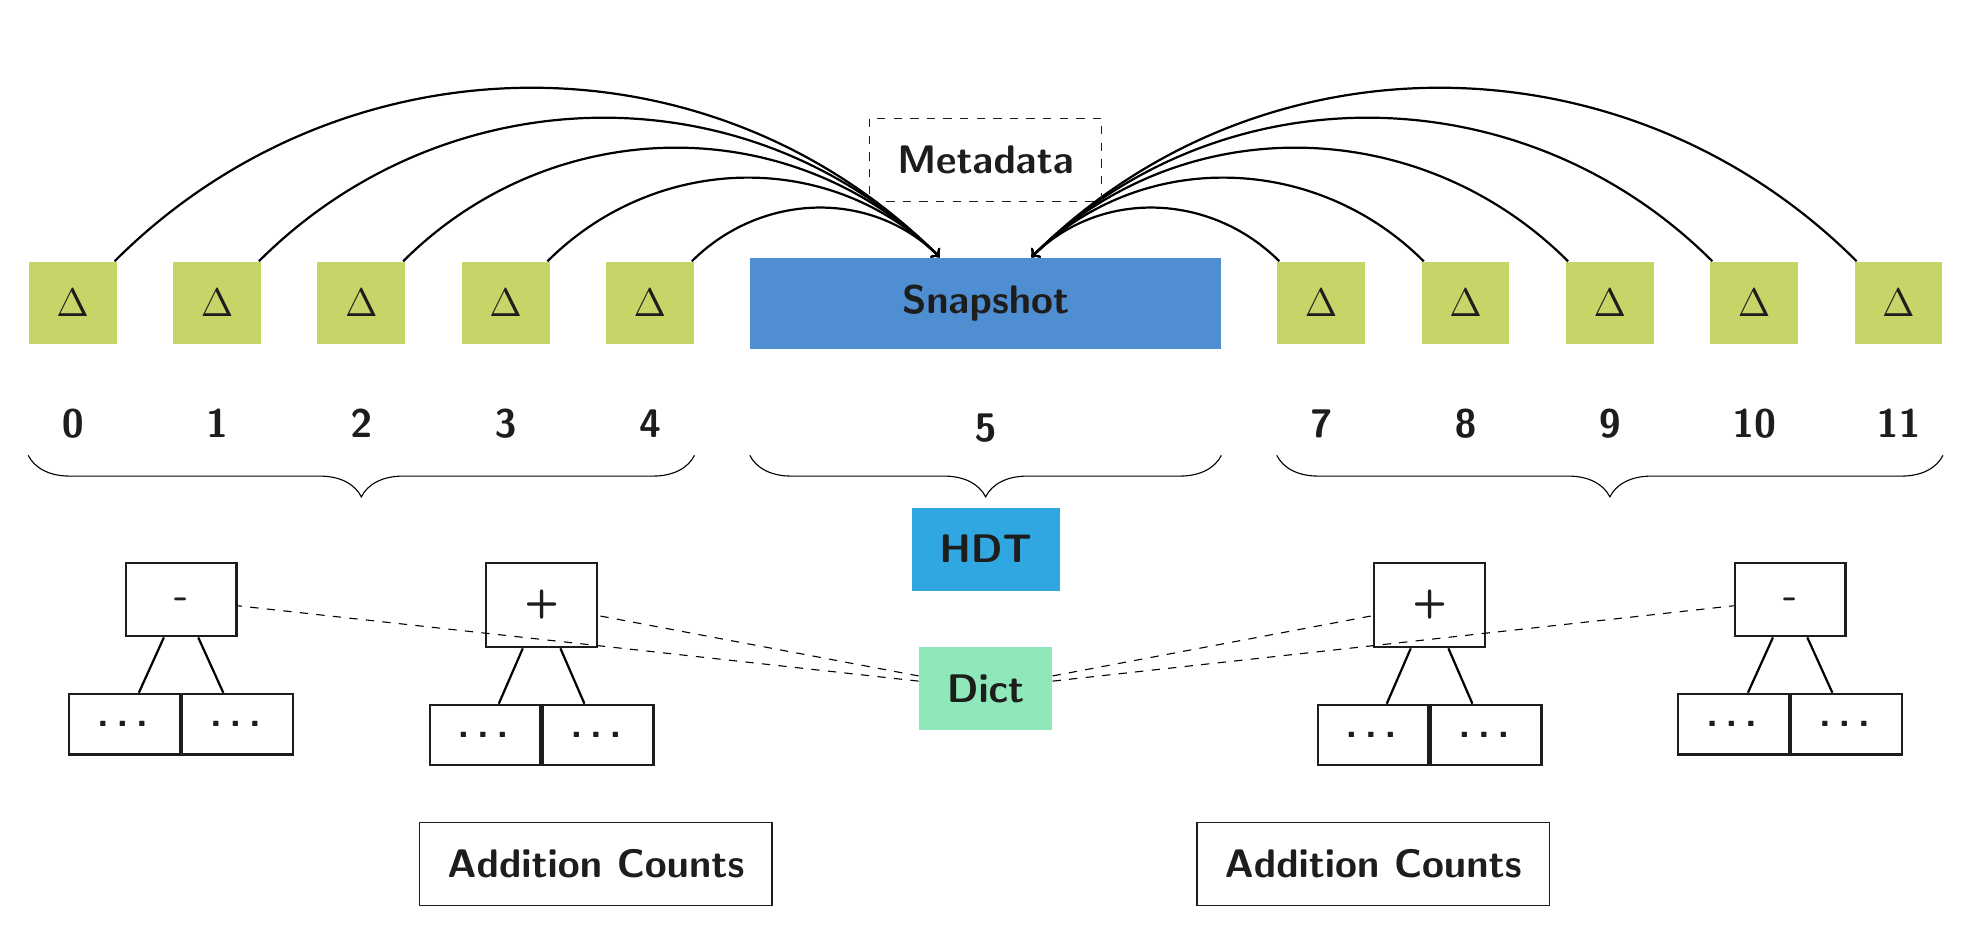
\begin{tikzpicture}[
    node distance = 2em, auto,
    font={\Large\itshape},
    base/.style={text=colortext,font={\Large\bfseries},inner sep=10pt,align=center,rectangle},
    txt/.style={text=colortext,font={\Large\bfseries},align=center},
    treenode/.style={base,thick,draw=colortext,text width=2em},
    relation/.style={text width=13em},
]

    % Nodes
    \node[base,fill=colorsnapshot,text width=15em] (snapshot) {Snapshot};
    \node[base,fill=colordelta,right=of snapshot]  (delta1)   {$\Delta$};
    \node[base,fill=colordelta,right=of delta1]    (delta2)   {$\Delta$};
    \node[base,fill=colordelta,right=of delta2]    (delta3)   {$\Delta$};
    \node[base,fill=colordelta,right=of delta3]    (delta4)   {$\Delta$};
    \node[base,fill=colordelta,right=of delta4]    (delta5)   {$\Delta$};
	\node[base,fill=colordelta,left=of snapshot]   (delta5r)  {$\Delta$};
	\node[base,fill=colordelta,left=of delta5r]    (delta4r)  {$\Delta$};
	\node[base,fill=colordelta,left=of delta4r]    (delta3r)  {$\Delta$};
	\node[base,fill=colordelta,left=of delta3r]    (delta2r)  {$\Delta$};
    \node[base,fill=colordelta,left=of delta2r]    (delta1r)  {$\Delta$};
    
    % Text
    \node[txt,below=of snapshot] (snaptxt)   {5};
    \node[txt,below=of delta1]               {7};
    \node[txt,below=of delta2]               {8};
    \node[txt,below=of delta3] (delta3txt)   {9};
    \node[txt,below=of delta4]               {10};
    \node[txt,below=of delta5]               {11};
    \node[txt,below=of delta1r]              {0};
    \node[txt,below=of delta2r]              {1};
    \node[txt,below=of delta3r] (delta3rtxt) {2};
    \node[txt,below=of delta4r]              {3};
    \node[txt,below=of delta5r]              {4};
    
    % Arrows
    \draw[->,thick](delta1) to [out=135,in=45] (snapshot);
    \draw[->,thick](delta2) to [out=135,in=45] (snapshot);
    \draw[->,thick](delta3) to [out=135,in=45] (snapshot);
    \draw[->,thick](delta4) to [out=135,in=45] (snapshot);
    \draw[->,thick](delta5) to [out=135,in=45] (snapshot);
    \draw[->,thick](delta1r) to [out=45,in=135] (snapshot);
    \draw[->,thick](delta2r) to [out=45,in=135] (snapshot);
    \draw[->,thick](delta3r) to [out=45,in=135] (snapshot);
    \draw[->,thick](delta4r) to [out=45,in=135] (snapshot);
    \draw[->,thick](delta5r) to [out=45,in=135] (snapshot);
    
    % Brace around snapshot and delta's
    \draw [decorate, decoration={brace,mirror,amplitude=15pt,raise=55pt}] (snapshot.west) -- (snapshot.east);
    \draw [decorate, decoration={brace,mirror,amplitude=15pt,raise=55pt}] (delta1.west) -- (delta5.east);
	\draw [decorate, decoration={brace,mirror,amplitude=15pt,raise=55pt}] (delta1r.west) -- (delta5r.east);
    
    % Dummy nodes for spacing
    \node[below=of delta3txt.south] (trees)      {};
    \node[left=of trees]            (treesleft)  {};
    \node[right=of trees]           (treesright) {};
    
    % Additions tree
    \node[treenode,below left=of treesleft] (additionsroot)        {+};
    \node[treenode,below=of additionsroot.south west] (additions1) {\ldots};
    \node[treenode,below=of additionsroot.south east] (additions2) {\ldots};
    \draw[-,thick](additions1) -- (additionsroot);
    \draw[-,thick](additions2) -- (additionsroot);
    
    % Deletions tree
    \node[treenode,below right=of treesright] (deletionsroot)      {-};
    \node[treenode,below=of deletionsroot.south west] (deletions1) {\ldots};
    \node[treenode,below=of deletionsroot.south east] (deletions2) {\ldots};
    \draw[-,thick](deletions1) -- (deletionsroot);
    \draw[-,thick](deletions2) -- (deletionsroot);
	
    % Addition Counts
    \node[base,draw=colortext,below=of additions1] (acounts) {Addition Counts};
	
    % Dummy nodes for spacing reverse
    \node[below=of delta3rtxt.south] (treesr)      {};
    \node[left=of treesr]            (treesrleft)  {};
    \node[right=of treesr]           (treesrright) {};
	
    % Additions tree reverse
    \node[treenode,below right=of treesrright] (additionsrroot)        {+};
    \node[treenode,below=of additionsrroot.south west] (additions1r) {\ldots};
    \node[treenode,below=of additionsrroot.south east] (additions2r) {\ldots};
    \draw[-,thick](additions1r) -- (additionsrroot);
    \draw[-,thick](additions2r) -- (additionsrroot);
    
    % Deletions tree r
    \node[treenode,below left=of treesrleft] (deletionsrroot)      {-};
    \node[treenode,below=of deletionsrroot.south west] (deletions1r) {\ldots};
    \node[treenode,below=of deletionsrroot.south east] (deletions2r) {\ldots};
    \draw[-,thick](deletions1r) -- (deletionsrroot);
    \draw[-,thick](deletions2r) -- (deletionsrroot);
	
    % Addition Counts reverse
    \node[base,draw=colortext,below=of additions1r,xshift=40pt] (acountsr) {Addition Counts};
    
    % HDT
    \node[base,fill=colorhdt,below=of snaptxt] (hdt) {HDT};
	
    % Dictionary
    \node[base,fill=colordict,below=of hdt] (dict) {Dict};
    \draw[-,dashed](dict) -- (additionsroot);
    \draw[-,dashed](dict) -- (deletionsroot);
    \draw[-,dashed](dict) -- (additionsrroot);
    \draw[-,dashed](dict) -- (deletionsrroot);
    
    % Metadata
    \node[base,dashed,draw=colortext,above=of snapshot] (meta) {Metadata};

\end{tikzpicture}
\end{document}
